%%
% Please see https://bitbucket.org/rivanvx/beamer/wiki/Home for obtaining beamer.
%%
\documentclass{beamer}
\RequirePackage[OT1]{fontenc}
\RequirePackage{amsthm,amsmath}
\RequirePackage[numbers]{natbib}
%\RequirePackage[colorlinks,linkcolor=blue,citecolor=blue,urlcolor=blue]{hyperref}
\usepackage{amssymb}
%\usepackage{anysize}
\usepackage{hyperref}
\usepackage{extarrows}
\usepackage{multirow}
\usepackage{natbib}
\usepackage{stmaryrd}
\usepackage{color}
\usepackage{soul}
%\usepackage[color=white]{todonotes}
\usepackage[disable]{todonotes}
\usepackage[perpage]{footmisc}
\usepackage{adjustbox}

\usepackage{wrapfig}
\usepackage{changepage}

% for tikz pictures
\usetikzlibrary{math}


%\usepackage{fontspec}
%\usepackage{arydshln}

\numberwithin{equation}{section}
\newtheorem{thm}{Theorem}[section]
\newtheorem{lem}[thm]{Lemma}
\newtheorem{pro}[thm]{Proposition}
\newtheorem{cor}[thm]{Corollary}
\newtheorem{defi}[thm]{Definition}
\newtheorem{rem}[thm]{Remark}
\newtheorem{assu}[thm]{Assumption}
\newtheorem{Exa}{Example}[section]
\newcommand{\be}{\begin{equation}}
\newcommand{\ee}{\end{equation}}
\newcommand{\bea}{\begin{eqnarray*}}
\newcommand{\eea}{\end{eqnarray*}}
\renewcommand*{\bibfont}{\footnotesize}

\newcommand{\eqby}[1]{\mathrel{\stackrel{#1}{=}}}
\newcommand{\eqbydef}{\mathrel{\stackrel{\hspace*{-3mm}\text{\tiny(def)}\hspace*{-3mm}}{=}}}
\newcommand{\leqby}[1]{\mathrel{\stackrel{#1}{\leq}}}
\newcommand{\geqby}[1]{\mathrel{\stackrel{#1}{\geq}}}
\newcommand{\deq}{\mathrel{\mathop:}=}
\newcommand\numberthis{\addtocounter{equation}{1}\tag{\theequation}} % use as in http://tex.stackexchange.com/questions/42726/align-but-show-one-equation-number-at-the-end
%\begin{align*}
%a &=b \\
%  &=c \numberthis \label{eqn}
%\end{align*}

\newcommand{\iid}[1]{\mathrel{\stackrel{\text{iid}}{\sim}}#1}
\newcommand{\iidnormal}{\mathrel{\stackrel{\text{iid}}{\sim}}\mathcal N(0,1)}

%\newcommand{\ofN}{^{(N)}}
\newcommand{\ofN}{}


\makeatletter
\newcommand{\biggg}{\bBigg@\thr@@}
\newcommand{\Biggg}{\bBigg@{3.5}}
\def\bigggl{\mathopen\biggg}
\def\bigggm{\mathrel\biggg}
\def\bigggr{\mathclose\biggg}
\def\Bigggl{\mathopen\Biggg}
\def\Bigggm{\mathrel\Biggg}
\def\Bigggr{\mathclose\Biggg}
\makeatother


\newcommand{\mR}{\mathbb R^n}
\makeatletter
\newcommand{\rmnum}[1]{\romannumeral #1}
\newcommand{\Rmnum}[1]{\expandafter\@slowromancap\romannumeral #1@}
\makeatother
\makeatletter % `@' now normal "letter"
\@addtoreset{equation}{section}
\makeatother  % `@' is restored as "non-letter"
\renewcommand\theequation{{\thesection}%
                   .{\arabic{equation}}}

\renewcommand{\thefootnote}{\fnsymbol{footnote}}
\newcommand{\abs}[1]{\lvert#1\rvert}

%    Blank box placeholder for figures (to avoid requiring any
%    particular graphics capabilities for printing this document).
\newcommand{\blankbox}[2]{%
  \parbox{\columnwidth}{\centering
%    Set fboxsep to 0 so that the actual size of the box will match the
%    given measurements more closely.
    \setlength{\fboxsep}{0pt}%
    \fbox{\raisebox{0pt}[#2]{\hspace{#1}}}%
  }%
}

\renewcommand{\baselinestretch}{1.2}





\newcommand{\fa}{{\frak a}} 
\newcommand{\bk}{{\bf{k}}}
\newcommand{\ttau}{\vartheta}

\newcommand{\LL}{L}
\newcommand{\fn}{{\mathfrak n}}

\newcommand{\wt}{\widetilde}
\newcommand{\wh}{\widehat}
\newcommand{\const}{\mbox{const}}
\newcommand{\La}{x}
\newcommand{\beqa}{\begin{eqnarray}}
\newcommand{\eeqa}{\end{eqnarray}}
%\newcommand{\e}{\varepsilon}
\newcommand{\eps}{\varepsilon}
\newcommand{\pt}{\partial}
\newcommand{\rd}{{\rm d}}
\newcommand{\bR}{{\mathbb R}}
\newcommand{\bC}{{\mathbb C}}

\newcommand{\bZ}{{\mathbb Z}}
\newcommand{\non}{\nonumber}
\newcommand{\wH}{{K}}


\newcommand{\bke}[1]{\left( #1 \right)}
\newcommand{\bkt}[1]{\left[ #1 \right]}
\newcommand{\bket}[1]{\left\{ #1 \right\}}
\newcommand{\norm}[1]{\| #1 \|}
\newcommand{\Norm}[1]{\left\Vert #1 \right\Vert}
\newcommand{\bka}[1]{\left\langle #1 \right\rangle}
\newcommand{\vect}[1]{\begin{bmatrix} #1 \end{bmatrix}}
\newcommand{\K}{n}
\newcommand{\z}{{\underline z}}
\renewcommand{\u}{{\underline u}}

\newcommand{\tr}{\mbox{tr\,}}



\newcommand{\unu}{{\underline {\nu}}}
\newcommand{\umu}{{\underline {\mu}}}


\renewcommand{\Re}{\mathsf{Re}\,}
\renewcommand{\Im}{\mathsf{Im}\,}
\newcommand{\supp}{\mathsf{supp}\,}

\newcommand{\ba}{{\bf{a}}}
\newcommand{\bb}{{\bf{b}}}
\newcommand{\bx}{{\bf{x}}}
\newcommand{\by}{{\bf{y}}}
\newcommand{\bu}{{\bf{u}}}
\newcommand{\bv}{{\bf{v}}}
\newcommand{\bw}{{\bf{w}}}
\newcommand{\bz}{{\bf {z}}}
\newcommand{\bq}{{\bf {q}}}
\newcommand{\tbx}{\widetilde\bx}
\newcommand{\bh}{{\bf{h}}}
\newcommand{\bn}{{\bf{n}}}

\newcommand{\fq}{{\frak q}}
\newcommand{\fu}{{\frak u}}
\newcommand{\bm}{{\bf  m }}
\newcommand{\bmu}{\mbox{\boldmath $\mu$}}
\newcommand{\sa}{{[\alpha ]}}


\newcommand{\tby}{\widetilde\by}

\newcommand{\bT}{{\T}}
\newcommand{\bO}{{\bf O}}

\newcommand{\bla}{\mbox{\boldmath $\lambda$}}
\newcommand{\bnu}{\mbox{\boldmath $\nu$}}
\newcommand{\bbeta}{\mbox{\boldmath $\beta$}}


\newcommand{\wG}{{\widehat G}}
\newcommand{\mg}{{m_H}}
\newcommand{\mW}{{m_W}}

\newcommand{\al}{\alpha}
\newcommand{\de}{\delta}




\newcommand{\barv}{ {[ v ]}}
\newcommand{\barZ}{ {[ Z ]}}

\newcommand{\ga}{{\gamma}}
\newcommand{\Ga}{{\Gamma}}
\newcommand{\la}{\lambda}
\newcommand{\Om}{{\Omega}}
\newcommand{\om}{{\omega}}
\newcommand{\si}{\sigma}
\renewcommand{\th}{\theta}
\newcommand{\td}{\widetilde}
\newcommand{\ze}{\zeta}

\newcommand{\cL}{{\mathscr L}}
\newcommand{\cE}{{\mathcal E}}
\newcommand{\cG}{{\mathcal G}}
\newcommand{\cX}{{\mathcal X}}
\newcommand{\cY}{{\mathcal Y}}
\newcommand{\cK}{{\mathcal K}}




\newcommand{\cM}{{\mathcal M}}
\newcommand{\cN}{{\mathcal N}}
\newcommand{\cH}{{\mathcal H}}
\newcommand{\cB}{{\mathcal B}}
\newcommand{\cU}{{\mathcal U}}

\newcommand{\bW}{{\bf W}}

\newcommand{\ov}{\overline}



%\newcommand{\re}{{\text Re \, }}
\newcommand{\re}{{\mathfrak{Re} \, }}
\newcommand{\im}{{\mathfrak{Im} \, }}
%\newcommand{\im}{{\text Im \, }}
\newcommand{\E}{{\mathbb E }}
\newcommand{\R}{{\mathbb R }}
\newcommand{\N}{{\mathbb N}}


\newcommand{\CC}{{\mathbb C }}
\newcommand{\RR}{{\mathbb R }}
\newcommand{\NN}{{\mathbb N}}
\newcommand{\g}{\gamma}
\newcommand{\ii}{\mathrm{i}}



\newcommand{\bl}{{\boldsymbol \lambda}}


\newcommand{\bt}{{\boldsymbol \theta}}
\newcommand{\htau}{{\hat\tau}}


\newcommand{\Ci}{{ C_{inf}}}
\newcommand{\Cs}{{ C_{sup}}}
\newcommand{\Z}{{\mathbb Z}}
\renewcommand{\P}{{\mathbb P}}


\newcommand{\C}{{\mathbb C}}
\newcommand{\pd}{{\partial}}

\newcommand{\nb}{{\nabla}}
\newcommand{\lec}{\lesssim}
\newcommand{\ind}{{\,\mathrm{d}}}

\renewcommand{\S}{\mathbb S}
\newcommand{\T}{\mathbb T}
\newcommand{\U}{\mathbb U}
\newcommand{\V}{\mathbb V}
\newcommand{\bU}{ {\bf  U}}
\newcommand{\bS}{ {\bf  S}}
\renewcommand{\S}{[\bf S]}

\newcommand{\ph}{{\varphi}}

\renewcommand{\div}{\mathop{\mathrm{div}}}
\newcommand{\curl}{\mathop{\mathrm{curl}}}
\newcommand{\spt}{\mathop{\mathrm{spt}}}
\newcommand{\wkto}{\rightharpoonup}
\newenvironment{pf}{{\bf Proof.}} {\hfill\qed}


\newcommand{\lv}{{\bar v}}
\newcommand{\lp}{{\bar p}}

\newcommand{\Cr}{\color{red}}
\newcommand{\Cb}{\color{blue}}
\newcommand{\Cg}{\color{green}}
\newcommand{\nc}{\normalcolor}

\renewcommand{\emph}[1]{{\Cr{#1}}}
\newcommand{\bemph}[1]{\textbf{\Cr{#1}}}

\newcommand{\e}{\varepsilon}

\title{Bounds on the Norm of Wigner-type Random Matrices}
\author{L\'aszl\'o Erd{\H{o}}s\inst{1} and Peter M{\"u}hlbacher\inst{1}}
\date{\today}
\institute[shortinst]{\inst{1} IST Austria}

\begin{document}

\begin{frame}
\titlepage
{\footnotesize Supported by ERC Advanced Grant No. 338804}
\end{frame}

%\begin{frame}
%\frametitle{Outline}
%\tableofcontents
%\end{frame}

\section{Introduction}
\begin{frame}
\frametitle{Central Question}
% random matrix = put probability measure on the space of NxN matrices; this naturally induces a random point process on the space of eigenvalues
% in general the assignment mapping matrix entries to eigenvalues is very complicated (for large dimensions N), but just like in the CLT we expect some "universal" behaviour in the sense that, under the right normalisation as N\to\infty, higher moments are forgotten/averaged out and universal patterns like the Gaussian occur
What can be said about the statistical properties of the eigenvalues of a large random matrix? (Wigner)

$$H=\begin{bmatrix}
    H_{11} & H_{12} & \dots  & H_{1N} \\
    H_{21} & H_{22} & \dots  & H_{2N} \\
    \vdots & \vdots & \ddots & \vdots \\
    H_{N1} & H_{N2} & \dots  & H_{NN}
\end{bmatrix} \Rightarrow (\lambda_1,\lambda_2,\dots,\lambda_N)\text{ eigenvalues}$$

$N =$ size of the matrix, will go to infinity.\\~

\emph{Analogy:} Central limit theorem. $\frac{X_1+\dots+X_N}{\sqrt N}\sim\mathcal N(0,\sigma^2)$ 
\end{frame}

\begin{frame}
\frametitle{Motivation}
% Wishart matrices are essentially a generalisation of the \Gamma distribution on the space of p.d. matrices and can be used to analyse sample covariance matrices
% ANNs have the same energy landscape as a p-spherical spin glass model with Hamiltonian $$H=H_{N,p} := N^{-(p-1)/2}\sum_{i_1,\dots,i_p=1}^N J_{i_1,\dots,i_p} \sigma_{i_1}\dots\sigma_{i_p}$$ for J_{i_1,\dots,i_p} ~ N(0,1)
% conditioning on some energy E, we have (under $\P(\cdot|H(\sigma)=E)$) that \nabla^2 H(\sigma) is equal in distribution to some deterministic f(N,p) times GOE --> shifted semicircle --> "layered structure", i.e. higher energy implies that Hessian has more negative eigenvalues (in probabilistic sense)
\begin{itemize}
	\item Physics
	\begin{itemize}
		\item nuclear physics (Wigner)
		\item mean field hopping mechanism with random transition rates
	\end{itemize}
	\item Statistics
	\begin{itemize}
		\item Wishart matrices
		\item sample covariance matrices
		\item neural networks (why are local minima good enough?)
	\end{itemize}
	\item ODEs with random coefficients
\end{itemize}
\end{frame}

\section{Setting}

\begin{frame}
\frametitle{Wigner type matrices}
% Wigner would be H_{ij} iid with S_{ij}=1/N
% we average in two ways: once by taking expectation, once by taking the arithmetic mean. so this is only a heuristic why this is the right normalisation, since it doesn't imply that any given eigenvalue is of order one.
% nonetheless it is a nice bound since it compares sth we hardly know anything about (eigenvalues) with sth that is given (S_{ij})
$H$ real-symmetric or complex hermitian $N\times N$ matrix\\
entries are \emph{centered} and \emph{independent} (up to $H_{ij}=\overline{H_{ji}}$ for $i\leq j$) with variance matrix $$S_{ij}\deq \E|H_{ij}|^2$$
such that $S_{ij}\leq\frac{C}{N}$ uniformly in $i,j$ for $C>0$ indep. of $N$.\\~


The eigenvalues $\lambda_1\leq \lambda_2\leq \dots\leq \lambda_N$ are of \emph{order one} (on average):
$$\E\frac{1}{N}\sum_i\lambda_i^2 = \E\frac{1}{N}Tr H^2 = \frac{1}{N}\sum_{ij}\E |H_{ij}|^2 = O(1)$$
\end{frame}


\begin{frame}
\frametitle{Density of States (DoS)}
% to state the main theorem we need to introduce some quantities that will be motivated later on
% expectation of empirical spectral density (still a measure that gives rise to a random variable!) is still hard to compute -> but it has been shown that \tilde\rho_N (a completely deterministic object, only depending on S!) is close to \E\rho_N
% convergence of measures here only in weak sense (empirical density is an atomic measure, whereas its expectation will have a density, so TV or other types of convergence will obviously fail)
Introduce the \emph{random measure}, referred to as \emph{empirical density}:
$$\rho_N\deq \frac{1}{N}\sum_{i=1}^N\delta_{\lambda_i}$$
Analogously to the \emph{law of large numbers} we have $$\rho_N\approx\E\rho_N,\quad\quad \text{for } N\gg 1$$
Under suitable higher moment assumptions we have that $$\E\rho_N \approx \widetilde\rho_N=\widetilde\rho_N(S)\quad\quad \text{for } N\gg 1,$$
where $\widetilde\rho_N\deq \displaystyle\lim_{\eta\downarrow 0} \frac{1}{\pi}\Im \langle{\bf m}(E+i\eta)\rangle$ is the inverse Stieltjes transform of $\mathbf m(z) = (m_1(z),\dots,m_N(z))$, the \emph{unique} (in $\mathbb H^N$) and \emph{deterministic} solution to $$-\frac{1}{m_x}=z+(Sm)_x,\quad x=1,\dots,N\quad\quad\quad\quad\quad \text{[QVE]}.$$
\end{frame}

\begin{frame}
\frametitle{Variance profile and density of states (DoS)}
% here we see that non-constant row-sums of S give rise to eigenvalue distributions other than the semicircle law
% possible questions: does it still have a density? (its only atomic component may be at zero.) is the density still convex? (no.) is the support still connected? (no.) is the density Hölder? (yes.)
\begin{figure}[hbt]
  \begin{tabular}{ccc}
   $\sum_i S_{ij}=1$ & $\Leftrightarrow$ & 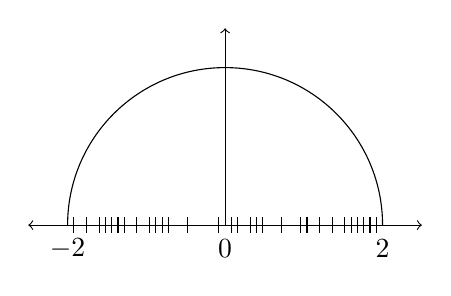
\begin{tikzpicture}[baseline=3ex]
		\begin{scope}
    		\clip (-2.05,0) rectangle (2.05,2.05);
    		\draw (0,0) circle(2);
		\end{scope}
		\draw[<->, thin] (-2.5,0) -- (2.5,0);
		\draw[->, thin] (0,0) -- (0,2.5);
		\node at (0,-0.3) {$0$};
		%\node at (0.4,2.3) {$\pi^{-1}$};
		\node at (-2,-0.3) {$-2$};
		\node at (2,-0.3) {$2$};
		\foreach \x in {-2,-1.92,...,2} {
			\tikzmath{\scx = (4-\x^2)^0.5/(2*3.14159265)-random(0,1);}
			\ifdim \scx pt > 0pt
				\draw[thin] (\x,-0.1) -- (\x,0.1);
			\fi}
		\end{tikzpicture}\\
   $\sum_i S_{ij}\neq 1$\\\begin{tikzpicture}[baseline=1ex]\node[inner sep=0pt]{\includegraphics[width=.3\textwidth]{generalvarianceprofile}};\end{tikzpicture} & $\Leftrightarrow$ & \begin{tikzpicture}[baseline=1ex]\node[inner sep=0pt]{\includegraphics[width=.4\textwidth]{generalDoS}};\end{tikzpicture}
  \end{tabular}
  \caption{General variance profile $S_{ij} \Rightarrow$ not the semicircle anymore.}
\end{figure}
\end{frame}

\section{Main result}

\begin{frame}
\frametitle{Main theorem}
% note that this is a completely deterministic statement, there are actually no random matrices here
% the z_j\leq 1 are the key parameters here, \leq because of submultiplicativity of the row-sum norm - note that this is not the spectral norm where this would always be one
% w_c(J)>1 and larger J gives larger w_c(J) -> better bound (both since z_j\leq 1 and the geometric series/its cutoff), but it's harder to compute with larger J
% \phi_J is essentially a polynomial for J large enough
% this gives an actual improvement because \|S^j\|\leq\|S\|^j hardly ever saturates
$S$ symmetric $N\times N$ matrix of variances, $J\in\N\cup\{\infty\}$, $z_j\deq\frac{\|S^j\|}{\|S\|^j}\leq 1$, where $\|S\|\deq\max_i\sum_j S_{ij}$, and $w_c(J)$ is the smallest positive root of the function $$
\phi_J(w):=1-\frac{w}{2}\Big(1+\sum_{j=1}^J\left(\frac{w}{2}\right)^jz_j+\sum_{j>J}\left(\frac{w}{2}\right)^j\Big).$$
	
	Then we have  $$\max\supp\widetilde\rho_N\leq 2\frac{\|S\|^\frac{1}{2}}{w_c(J)}.$$

\bemph{Comparison to existing literature:} 
\begin{itemize}
	\item ~\!\![Ajanki-Erd{\H{o}}s-Kr{\"u}ger 2015]: $\max\supp\widetilde\rho_N\leq 2\|S\|^\frac{1}{2}$.
	\item ~\!\![Ottolino 2017]: exact expression for $\max\supp\widetilde\rho_N$ in terms of a variational formula of $S$; our approach is different since it gives an explicit bound only in terms of powers of $S$.
\end{itemize}

\end{frame}

\begin{frame}
\frametitle{Corollary}
% this is a corollary from Laszlo's work (--> does not follow from our result using elementary steps!), which links the support of \tilde\rho_N to the distribution of the largest eigenvalue
% finite moment assumption necessary just like in CLT to bound some random quantity in the large N limit by some deterministic object depending only on the first two moments
This follows using \emph{local laws} from [Erd{\H o}s,  Kr\"uger,  Schr\"oder, 2017].
Let $H=H^{(N)}$ be a sequence of Wigner type matrices with variance matrices $S=S^{(N)}$, set $$
 z_j:= \limsup_{N\to\infty}  \frac{\|[S^{(N)}]^j\|}{\|S^{(N)}\|^j}\leq 1
$$
and for any $J\in \N \cup\{\infty\}$ let $w_c(J)$ the smallest positive root of $\phi_J$.


Under \emph{finite moment assumption}: $$\forall q\in\N:\exists C_q : \E \max_{i,j,N}(\sqrt N |H_{ij}|)^q\leq C_q,$$
for any $\epsilon>0$ (small) and any $D>0$ (large) we have the following bound on the largest eigenvalue of $H$:
$$
  {\color{red}\P \Big(  |\lambda_{max} (H^{(N)})|\ge 2\frac{\|S^{(N)}\|^\frac{1}{2}}{w_c(J)} +\epsilon\Big)  \le C(\epsilon, D) N^{-D}}
 $$
 for $C(\epsilon, D) = C(\epsilon, D, C^*,(C_q)_q)$ with $C^*$ such that $S_{ij}\leq\frac{C^*}{N}$.

\end{frame}

\begin{frame}
\frametitle{Numerics}
% few samples of H=H^{(N)} are needed because of the concentration of measure phenomenon
\begin{figure}[hbt]
  \includegraphics[scale=0.3]{numVarProfile}
  \caption{Variance profile $S_{ij}= \frac{1}{N} e^{\frac{i+j}{N}}$ for $N=500$.}
\end{figure}
\begin{itemize}
	\item The already known bound yields {\color{red}$2\|S\|^{1/2}\approx 4.316$}.
	\item For $J=50$ our bound gives {\color{red}$2\|S\|^\frac{1}{2}/w_c \approx 3.870$}, an improvement by a factor of $w_c \approx 1.115$.
	\item The empirical average (number of samples = 10) of the largest eigenvalue (in absolute value) is {\color{red}$\approx 3.677$} (with empirical standard deviation of $\approx 0.047$)
\end{itemize}
\end{frame}

\section{Relating spectral density to QVE}

\begin{frame}
\frametitle{How to get the DoS in terms of $S$ - Stieltjes transform}
% remember that \tilde\rho_N was defined as inverse Stieltjes transform, so let's define the Stieltjes transform first
% the takeaway from this slide are two statements:
%  1: the imaginary part of the Stieltjes transform is essentially a convolution with the Poisson kernel that converges to a delta distribution as the imaginary part of the argument goes to zero --> hence immediately get the inverse Stieltjes transform
%  2: (technical) conditions for a Herglotz function to be a Stieltjes transform of some real measure
\bemph{Definition} Let $\mu$ be a probability measure on $\R$. Its \emph{Stieltjes transform} $m_\mu:\mathbb H\to \C$ is given by $$m_\mu(z)\deq \int_\R \frac{d\mu(x)}{x-z}$$
\bemph{Properties}\begin{itemize}
	\item $z\mapsto m_\mu(z)$ is analytic in $\mathbb H$ with image in $\mathbb H$: $$\Im m_\mu(E+i\eta)=\eta\int_\R \frac{d\mu(x)}{(x-E)^2+\eta^2} = (\pi\mu * P_\eta)(E),$$
	where $P_\eta(x)\deq \frac{1}{\pi}\frac{\eta}{x^2+\eta^2}$ is the Poisson kernel, satisfying \begin{itemize}\item $\int_\R P_\eta(x)dx=1$ \item $P_\eta(E) \wkto \delta_E$ as $\eta\downarrow 0$ \end{itemize}
	\item For every analytic $m:\mathbb H\to\mathbb H$ with $i\eta m(i\eta)\to -1$ as $\eta\to \infty$ and $|m(z)|\leq \frac{1}{\Im(z)}$ there is a measure $\mu$ such that $$\frac{1}{\pi}\Im m(\cdot+i\eta) \wkto \mu\quad\quad \text{as }\eta\downarrow 0$$
\end{itemize}
\end{frame}

\begin{frame}
\frametitle{How to get the DoS in terms of $S$ - resolvents}
% correspondence between Stieltjes transform and Tr of resolvent is trivial by spectral theorem
% this allows us to _completely_ encode the spectral density in Tr G, provided we can do the inverse Stieltjes transform
\bemph{Obvious:} Trace of the resolvent $G$ of a hermitian matrix $H$ is the Stieltjes transform of its empirical spectral density.
$$\rho_N\eqbydef \frac{1}{N}\sum_{i=1}^N\delta_{\lambda_i},\quad\quad m_{\rho_N}(z)\eqbydef \frac{1}{N}\sum_{i=1}^N\frac{1}{\lambda_i-z}\eqbydef \frac{1}{N}Tr G(z)$$
While, in general, $$\lim_{\eta\downarrow 0}\Im m_{\rho_N}(E+i\eta)$$ does not exist, its expectation may exist $$\rho(E)\deq \lim_{\eta\downarrow 0}\E \Im m_{\rho_N}(E+i\eta)$$
and gives the \emph{density of states (DoS)} $\rho$.
\end{frame}

\begin{frame}
\frametitle{How to get the DoS in terms of $S$ - resolvents}
% m is a unique solution if we restrict ourselves to functions mapping H _to H_
% why is m interesting? because it is close to the main diagonal of the resolvent --> Tr G can be written as average of m --> have Stieltjes transform of spectral density
% criteria for existence of inverse Stieltjes transform for this average of m can be checked
% note: off diagonal entries of the resolvent typically vanish as N\to\infty under quite general assumptions
\bemph{Highly non-trivial:} For $\mathbf m(z) = (m_1(z),\dots,m_N(z))$ the \emph{unique} and \emph{deterministic} solution in $\mathbb H^N$ to $$-\frac{1}{m_x}=z+(Sm)_x,\quad x=1,\dots,N\quad\quad\quad\quad\quad \text{[QVE]}$$ it is shown in [Ajanki-Erd{\H{o}}s-Kr{\"u}ger 2015] that $$G(z)\eqbydef \frac{1}{H-z},\quad\quad G_{xx}(z) \approx m_x(z),\quad\quad\text{as }N\to\infty$$
So \emph{to compute the DoS} for $H$, we need to \emph{solve the QVE} for every $z\in\mathbb H$ and compute the inverse Stieltjes transform of $$\langle\mathbf m(z)\rangle\deq \frac{1}{N}\sum_x m_x(z).$$
\end{frame}

\section{Relating QVE to trees}

\begin{frame}
\frametitle{Solving the QVE}
% Wigner case (/sth slightly more general): the r.h.s. is independent of i, hence the l.h.s. is as well --> the QVE simplifies to a quadratic scalar equation which we can solve explicitly to get Wigner's semicircle law (after applying the inverse Stieltjes transform) --> proof of concept (since \tilde\rho_N = Stieltjes transform of WCSL for all N, even for small N!)
% general case: more complicated. introduce shortcut u_x (will be more convenient to work with) and write it in a way without fractions (by geometric series) and recursively plug it into itself to get general form of m_x
% from that form it can be read of that DoS is still symmetric --> justifies only looking for the largest eigenvalue
\bemph{Case} $S_{ij}=\frac{1}{N}$:
$$-\frac{1}{m_x}\eqbydef z+(Sm)_x = z+\langle\mathbf m\rangle, \quad \forall i$$
thus $m_x=\langle\mathbf m\rangle$ and $-\frac{1}{\langle\mathbf m\rangle}=z+\langle\mathbf m\rangle$ which gives the \emph{semicircle law}.

\bemph{Case} $S_{ij}\neq\frac{1}{N}$: Note that [QVE] is equivalent to $$-zm_x=:u_x = \frac{1}{1-\frac{1}{z^2}(Su)_x} = \sum_{n=0}^\infty z^{-2n}\left(\sum_{y=1}^N S_{xy}u_y\right)^n\quad\quad (*)$$
Immediate by recursively plugging in $(*)$: $$m_x = -\frac{1}{z}\sum_{n=0}^\infty c_{n,x}z^{-2n},\quad c_{n,x}\in\R$$ $\Rightarrow$ $-\overline{m_x(z)} = m_x(-\bar z)$ $\Rightarrow$ $\Im\langle\mathbf m(E+i\eta)\rangle=\Im\langle\mathbf m(-E+i\eta)\rangle$ $\Rightarrow$\;DoS symmetric
\end{frame}



\begin{frame}
\begin{adjustwidth}{-0.7cm}{}
\frametitle{Solving the QVE}
% just plugging in u_x into itself and every time you do that, add an edge to the tree representation
% n(x) is just a dummy variable, dependence on x just to keep track for which vertex we are selecting how many children it gets
For \begin{tikzpicture}[baseline = 1ex, scale=.5]
   			\draw[dashed] (0,0) -- (0,1);
   			\draw[fill=white] (0,0) circle (3pt);
   		\end{tikzpicture} $\deq \frac{1}{z^2}\sum_{y=1}^N S_{xy}u_y$,
   		\begin{tikzpicture}[baseline = 1ex, scale=.5]
   			\draw[dashed] (.5,1) -- (0,0) -- (-.5,1);
   			\draw[fill=white] (0,0) circle (3pt);
   		\end{tikzpicture} $\deq \Big($ \begin{tikzpicture}[baseline = 1ex, scale=.5]
   			\draw[dashed] (0,0) -- (0,1);
   			\draw[fill=white] (0,0) circle (3pt);
   		\end{tikzpicture} $\Big)^2, \dots,$  we have
\begin{figure}[h]
	\begin{tabular}{ccc}
		\begin{tikzpicture}[baseline = 1ex, scale=.5]
   			\draw[fill=white] (0,0) circle (3pt);
   		\end{tikzpicture} + 
   		\begin{tikzpicture}[baseline = 1ex, scale=.5]
   			\draw[dashed] (0,0) -- (0,1);
   			\draw[fill=white] (0,0) circle (3pt);
   		\end{tikzpicture} + 
   		\begin{tikzpicture}[baseline = 1ex, scale=.5]
   			{\color<2->{red}
   			\draw[dashed] (.5,1) -- (0,0) -- (-.5,1);
   			\draw[fill=white] (0,0) circle (3pt);}
   		\end{tikzpicture} + 
   		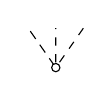
\begin{tikzpicture}[baseline = 1ex, scale=.5]
   			\draw[dashed] (.7,1) -- (0,0) -- (-.7,1) -- (0,0) -- (0,1);
   			\draw[fill=white] (0,0) circle (3pt);
   		\end{tikzpicture} + $\dots$ & $\Leftrightarrow$
   		& {\small $\displaystyle{\sum_{n(x)=0}^\infty z^{-2n(x)}\left(\sum_y S_{xy}u_y\right)^{n(x)}\eqbydef u_x}$} \\
	\uncover<2->{
   		{\small (choose $n(x)=2$)} & & $\Downarrow$ \\
   		
\begin{tikzpicture}[baseline = 1ex, scale=.5]
   			\draw[thick] (.5,1) -- (0,0) -- (-.5,1);
   			\draw[fill=white] (0,0) circle (3pt);
   			\draw[fill=black] (-.5,1) circle (3pt);
   			\draw[fill=black] (.5,1) circle (3pt);
   		\end{tikzpicture} + 
   		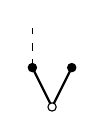
\begin{tikzpicture}[baseline = 1ex, scale=.5]
   			\draw[thick] (.5,1) -- (0,0) -- (-.5,1);
   			\draw[dashed] (-.5,1) -- (-.5,2);
   			\draw[fill=white] (0,0) circle (3pt);
   			\draw[fill=black] (-.5,1) circle (3pt);
   			\draw[fill=black] (.5,1) circle (3pt);
   		\end{tikzpicture} + 
   		\begin{tikzpicture}[baseline = 1ex, scale=.5]
   			{\color<4->{red}
   			\draw[thick] (.5,1) -- (0,0) -- (-.5,1);
   			\draw[dashed] (.5,1) -- (.5,2);
   			\draw[fill=white] (0,0) circle (3pt);
   			\draw[fill=black] (-.5,1) circle (3pt);
   			\draw[fill=black] (.5,1) circle (3pt);
   			}
   		\end{tikzpicture} + 
   		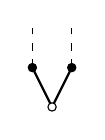
\begin{tikzpicture}[baseline = 1ex, scale=.5]
   			\draw[thick] (.5,1) -- (0,0) -- (-.5,1);
   			\draw[dashed] (-.5,1) -- (-.5,2);
   			\draw[dashed] (.5,1) -- (.5,2);
   			\draw[fill=white] (0,0) circle (3pt);
   			\draw[fill=black] (-.5,1) circle (3pt);
   			\draw[fill=black] (.5,1) circle (3pt);
   		\end{tikzpicture} + $\dots$ & $\Leftrightarrow$ & 
   			\only<2>{\small $\displaystyle{z^{-4}\underbrace{\left(\sum_{a}S_{xa}u_a\right)^2}_{\sum_{a_1a_2}S_{xa_1}S_{xa_2}u_{a_1}u_{a_2}}}$}
   			\only<3->{\tiny $\displaystyle{\!\!\!\!\!\!\!\frac{1}{z^4}\sum_{a_1a_2}S_{xa_1}\!S_{xa_2}\!\!\left[\sum_{n(a_1)}\left(\frac{1}{z^2}\sum_b S_{a_1b}u_b\right)^{n(a_1)}\right]\left[\sum_{n(a_2)}\dots\right]}$} \\
    }
\uncover<4->{
   		{\small (choose $n(a_1)=0,n(a_2)=1$)} & & $\Downarrow$ \\
   		\begin{tikzpicture}[baseline = 2.5ex, scale=.5]
   			{\color<6->{red}
   			\draw[thick] (-.5,1) -- (0,0) -- (.5,1) -- (.5,2);
   			\draw[fill=white] (0,0) circle (3pt);
   			\draw[fill=black] (-.5,1) circle (3pt);
   			\draw[fill=black] (.5,1) circle (3pt);
   			\draw[fill=black] (.5,2) circle (3pt);
   			}
   		\end{tikzpicture} + 
   		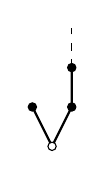
\begin{tikzpicture}[baseline = 2.5ex, scale=.5]
   			\draw[thick] (-.5,1) -- (0,0) -- (.5,1) -- (.5,2);
   			\draw[dashed] (.5,2) -- (.5,3);
   			\draw[fill=white] (0,0) circle (3pt);
   			\draw[fill=black] (-.5,1) circle (3pt);
   			\draw[fill=black] (.5,1) circle (3pt);
   			\draw[fill=black] (.5,2) circle (3pt);
   		\end{tikzpicture} + 
   		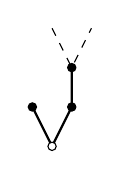
\begin{tikzpicture}[baseline = 2.5ex, scale=.5]
   			\draw[thick] (-.5,1) -- (0,0) -- (.5,1) -- (.5,2);
   			\draw[dashed] (0,3) -- (.5,2) -- (1,3);
   			\draw[fill=white] (0,0) circle (3pt);
   			\draw[fill=black] (-.5,1) circle (3pt);
   			\draw[fill=black] (.5,1) circle (3pt);
   			\draw[fill=black] (.5,2) circle (3pt);
   		\end{tikzpicture} + $\dots$ & $\Leftrightarrow$ & 
   			\only<4>{\small $\displaystyle{\frac{1}{z^{2(2+0+1)}} \sum_{a_1a_2b}S_{xa_1}S_{xa_2}S_{a_2b}u_b}$}
   			\only<5->{\small $\displaystyle{\frac{1}{z^6}\sum_{a_1a_2b}S_{xa_1}S_{xa_2}S_{a_2b}\uncover<5>{u_b}}$} \\
    }
    \uncover<5>{
    	$\vdots$ & & $\vdots$
    }
  \end{tabular}
\end{figure}
\end{adjustwidth}
\end{frame}

\begin{frame}
\frametitle{Defining the value of a tree}
% introduce dummy labels for vertices of a tree to sum over
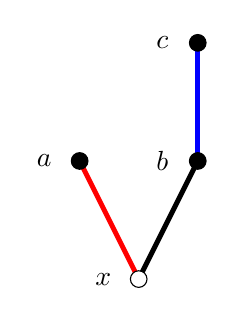
\begin{tikzpicture}[baseline = 8ex, scale=1.5]

	{\color{red} \draw[line width=1.8pt] (-.5,1) -- (0,0);}
	{\color{black} \draw[line width=1.8pt] (0,0) -- (.5,1);}
	{\color{blue} \draw[line width=1.8pt] (.5,1) -- (.5,2);}
	\draw[fill=white] (0,0) circle (2pt);
	\draw[fill=black] (-.5,1) circle (2pt);
	\draw[fill=black] (.5,1) circle (2pt);
	\draw[fill=black] (.5,2) circle (2pt);
	
	\node at (-0.3,0) {$x$};
	\node at (-0.8,1) {$a$};
	\node at ( 0.2,1) {$b$};
	\node at ( 0.2,2) {$c$};
\end{tikzpicture} $\quad\quad\Leftrightarrow\quad\quad$ $\displaystyle{\sum_{a,b,c}{\color{red} S_{xa}}{\color{black} S_{xb}}{\color{blue} S_{bc}} = val_x\Bigg(}$ 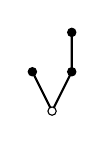
\begin{tikzpicture}[baseline = 2.5ex, scale=.5]
   			\draw[thick] (-.5,1) -- (0,0) -- (.5,1) -- (.5,2);
   			\draw[fill=white] (0,0) circle (3pt);
   			\draw[fill=black] (-.5,1) circle (3pt);
   			\draw[fill=black] (.5,1) circle (3pt);
   			\draw[fill=black] (.5,2) circle (3pt);
	\end{tikzpicture} $\Bigg)$
\\~\\
\emph{Note:} \begin{itemize}
	\item sum only over (the labels of) unfilled vertices
	\item $n$ edges encode factor of $\frac{1}{z^{2n}}$
\end{itemize}

Formalize this notation by assigning to each \emph{rooted, planar tree with $n$ edges} $\Gamma\in\mathcal T_n$ its value: $$val\ofN_x(\Gamma)\deq \Big(\prod_{v\in V(\Gamma)}\sum_{x_v=1}^N\Big)\Big[\delta_{x_\text{root}=x} \prod_{e\in E(\Gamma)}S_{x_{e_-}x_{e_+}}\Big].$$
\end{frame}


\begin{frame}
\frametitle{Relating trees to DoS}
% the takeaway here is that, in order to bound the support of the DoS, it suffices to bound coefficients of large powers of z, i.e. know the contribution of large trees
% we can't bound non-linear trees well, so we somehow need to "linearise" our trees in order to bound their contribution by row-sum norms of suitably chosen powers of S
Applying that procedure recursively yields the following \bemph{Proposition}:
	$$m_x\ofN(z)=-\frac{1}{z}\sum_{n=0}^\infty \Big[\sum_{\Gamma\in\mathcal T_n}val\ofN_x(\Gamma)\Big]z^{-2n}.{\quad\quad\quad\qed}$$
	
\hrulefill
\begin{itemize}
	\item[recall:] (average of) $m_x$ is the Stieltjes transform of DoS
	\item[note:] $m_\mu$ Stieltjes transform of $\mu$ $\Rightarrow$ $m_\mu$ analytic in $\C\setminus\supp\mu$
	\item [$\Rightarrow$] $\displaystyle{\max\supp\rho\ofN\leq \limsup_n\Bigg|\sum_{\Gamma\in\mathcal T_n}\max_xval_x\ofN(\Gamma)\Bigg|^\frac{1}{2n}}$ {\small by Cauchy-Hadamard}
	\item [note:] cannot bound $val_x(\Gamma)$ unless $\Gamma$ is linear $\Rightarrow$ $val_x(\Gamma) = \sum_i(S^n)_{xi}$
\end{itemize}
\end{frame}

\begin{frame}
\frametitle{Bounding $val(\Gamma)\deq \max_xval(\Gamma)$}
% we can "linearise" trees by "chopping them up" (this corresponds to taking max over cleverly chosen dummy variables
% note that an unfilled vertex indicates that we're taking max over its label, a filled vertex indicates that we're summing over its label
% we will use three kinds of splittings: rightmost, leftmost, complete
$\displaystyle{val\ofN\Bigg(}$\!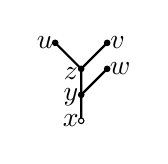
\begin{tikzpicture}[baseline=2ex, scale=.33]
		%% vertex labels
		\node at (-0.4,0) {$x$};
		\node at (-0.4,.9) {$y$};
		\node at (-0.4,1.8) {$z$};
		\node at (-1.4,3) {$u$};
		\node at (1.4,3) {$v$};
		\node at (1.5,2) {$w$};
		%% edges
		\draw[thick] (0,0) -- (0,1) -- (0,2) -- (-1,3);
		\draw[thick] (0,2) -- (1,3);
		\draw[thick] (0,1) -- (1,2);
		%% vertices
		\draw[fill=white] (0,0) circle (3pt);
		\draw[fill=black] (0,1) circle (3pt);
		\draw[fill=black] (0,2) circle (3pt);
		\draw[fill=black] (-1,3) circle (3pt);
		\draw[fill=black] (1,3) circle (3pt);
		\draw[fill=black] (1,2) circle (3pt);
	\end{tikzpicture}\!\!$\displaystyle{\Bigg)\eqbydef\max_x \sum_{yzuvw} S_{xy}S_{yz}S_{zu} S_{zv}S_{yw}\uncover<3->{\leq \|S\|^5}}$ \uncover<3->{$\Leftrightarrow$ \!\!\!\!\!\!\!\!\!\!\!\!\!\!\!\!\!\!\!\!\!\!\!\!	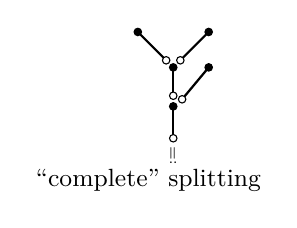
\begin{tikzpicture}[scale=0.45,baseline=3ex]
		%% edges
		\draw[thick] (0,0) -- (0,1);
		\draw[thick] (0,1.2) -- (0,2);
		\draw[thick] (-0.2,2.2) -- (-1,3);
		\draw[thick] (0.2,2.2) -- (1,3);
		\draw[thick] (0.25,1.1) -- (1,2);		
		%% vertices
		\draw[fill=white] (0,0) circle (3pt);
		\draw[fill=black] (0,.9) circle (3pt);
		\draw[fill=white] (0,1.2) circle (3pt);
		\draw[fill=white] (0.25,1.1) circle (3pt);
		\draw[fill=black] (0,2) circle (3pt);
		\draw[fill=white] (-0.2,2.2) circle (3pt);
		\draw[fill=white] (0.2,2.2) circle (3pt);
		\draw[fill=black] (-1,3) circle (3pt);
		\draw[fill=black] (1,3) circle (3pt);
		\draw[fill=black] (1,2) circle (3pt);
		{\tiny \node[rotate=90] at (0,-.5) {:=};}
		{\small \node at (-.7,-1.2) {``complete" splitting};}
	\end{tikzpicture}\vspace{-.5cm}\!\!\!\!\!\!\!\!\!\!\!\!}

\begin{figure}[hbt]
  \begin{tabular}{rcc}
   \only<1>{
   $\displaystyle{
   		\leq \max_x \sum_{yzu} S_{xy}S_{yz}S_{zu}\max_{z'} \sum_v S_{z'v} \max_{y'} \sum_w S_{y'w}
   	}$}
   \only<2->{
   $\displaystyle{
   		\leq \|S^3\| \|S\|^2
   	}$
   }
   
    & $\Leftrightarrow$ & 
    
    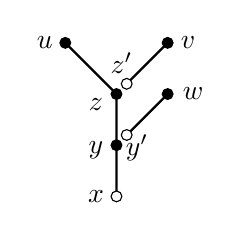
\begin{tikzpicture}[baseline=4ex, scale=.65]
		%% vertex labels
		\node at (-0.4,0) {$x$};
		\node at (-0.4,.9) {$y$};
		\node at (0.4,.95) {$y'$};
		\node at (-0.4,1.8) {$z$};
		\node at (.1,2.6) {$z'$};
		\node at (-1.4,3) {$u$};
		\node at (1.4,3) {$v$};
		\node at (1.5,2) {$w$};
		%% edges
		\draw[thick] (0,0) -- (0,1) -- (0,2) -- (-1,3);
		\draw[thick] (0.2,2.2) -- (1,3);
		\draw[thick] (0.2,1.2) -- (1,2);		
		%% vertices
		\draw[fill=white] (0,0) circle (3pt);
		\draw[fill=black] (0,1) circle (3pt);
		\draw[fill=white] (0.2,1.2) circle (3pt);
		\draw[fill=black] (0,2) circle (3pt);
		\draw[fill=white] (0.2,2.2) circle (3pt);
		\draw[fill=black] (-1,3) circle (3pt);
		\draw[fill=black] (1,3) circle (3pt);
		\draw[fill=black] (1,2) circle (3pt);
	\end{tikzpicture}
	\only<2->{$=:$ ``leftmost" splitting}\\
   \only<1>{
   $\displaystyle{
   		\leq \max_x \sum_{yw} S_{xy}S_{yw} \max_{y'} \sum_{zv} S_{y'z}S_{zv} \max_{z'} \sum_u S_{z'u}
   	}$}
   \only<2->{
   $\displaystyle{
   		\leq \|S^2\|^2 \|S\|
   	}$
   }
   
    & $\Leftrightarrow$ & 
    
    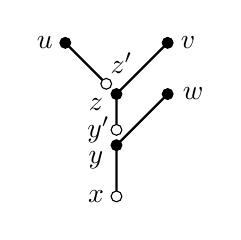
\begin{tikzpicture}[baseline=4ex, scale=.65]
		%% vertex labels
		\node at (-0.4,0) {$x$};
		\node at (-0.35,1.3) {$y'$};
		\node at (-0.4,.7) {$y$};
		\node at (-0.4,1.8) {$z$};
		\node at (.1,2.6) {$z'$};
		\node at (-1.4,3) {$u$};
		\node at (1.4,3) {$v$};
		\node at (1.5,2) {$w$};
		%% edges
		\draw[thick] (0,0) -- (0,1) -- (1,2);
		\draw[thick] (0,1.2) -- (0,2) -- (1,3);
		\draw[thick] (-0.2,2.2) -- (-1,3);
		%% vertices
		\draw[fill=white] (0,0) circle (3pt);
		\draw[fill=black] (0,1) circle (3pt);		
		\draw[fill=white] (0,1.3) circle (3pt);
		\draw[fill=black] (0,2) circle (3pt);
		\draw[fill=white] (-0.2,2.2) circle (3pt);
		\draw[fill=black] (-1,3) circle (3pt);
		\draw[fill=black] (1,3) circle (3pt);
		\draw[fill=black] (1,2) circle (3pt);
	\end{tikzpicture}
	\only<2->{$=:$ ``rightmost" splitting}\\
  \end{tabular}
  
  {\small The unfilled vertex indicates we are taking the maximum over this vertex'\,label instead of summing over it.}
\end{figure}

\end{frame}

\begin{frame}
\frametitle{Calculating $\sum_{\Gamma\in\mathcal T_n}val(\Gamma)$ for fixed $n\gg 1$}
% write the sum of values over trees as expectation w.r.t. uniform measure --> this brings us back to a probabilistic setting
% uniform measure over trees with given number of edges is hard, but luckily there's a correspondence between Dyck paths and these trees --> (how) does the chopping-up translate to the Dyck path representation?
For $\E$ the expectation under the uniform measure on $\mathcal T_n$: $$\sum_{\Gamma\in\mathcal T_n}val(\Gamma) = |\mathcal T_n|\;\E val(\Gamma)$$

\begin{itemize}
	\item $\lim_{n\to\infty} |\mathcal T_n|^\frac{1}{2n}=2$
	\item define Dyck paths of length $2n$: $$\!\!\!\!\!\!\!\!\!\!\!\!\!\!\!\!D_{2n}\deq \{\pi: [0,2n]\cap\N \to \N : \pi(0)=\pi(2n)=0 \text{ and }|\pi(i)-\pi(i+1)|=1\}$$
	\item there is a bijection between \emph{Dyck paths} $D_{2n}$ and $\mathcal T_n$:\quad
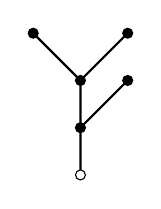
\begin{tikzpicture}[baseline=4ex, scale=.6]
		%% edges
		\draw[thick] (0,0) -- (0,1) -- (0,2) -- (-1,3);
		\draw[thick] (0,2) -- (1,3);
		\draw[thick] (0,1) -- (1,2);
		%% vertices
		\draw[fill=white] (0,0) circle (3pt);
		\draw[fill=black] (0,1) circle (3pt);
		\draw[fill=black] (0,2) circle (3pt);
		\draw[fill=black] (-1,3) circle (3pt);
		\draw[fill=black] (1,3) circle (3pt);
		\draw[fill=black] (1,2) circle (3pt);
	\end{tikzpicture}
$\Leftrightarrow$%\!\!\!\!\!
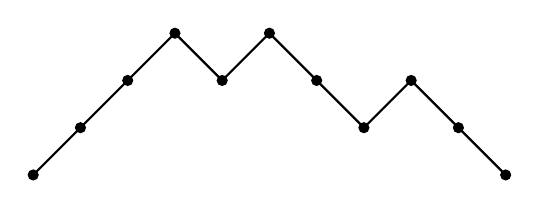
\begin{tikzpicture}[baseline=4ex, scale=.6]
	%% vertices
	\draw[fill=black] (0,0) circle (3pt);
	\draw[fill=black] (1,1) circle (3pt);
	\draw[fill=black] (2,2) circle (3pt);
	\draw[fill=black] (3,3) circle (3pt);
	\draw[fill=black] (4,2) circle (3pt);
	\draw[fill=black] (5,3) circle (3pt);
	\draw[fill=black] (6,2) circle (3pt);
	\draw[fill=black] (7,1) circle (3pt);
	\draw[fill=black] (8,2) circle (3pt);
	\draw[fill=black] (9,1) circle (3pt);
	\draw[fill=black] (10,0) circle (3pt);
	\draw[thick] (0,0) -- (1,1) -- (2,2) -- (3,3) -- (4,2) -- (5,3) -- (6,2) -- (7,1) -- (8,2) -- (9,1) -- (10,0);
\end{tikzpicture}

\end{itemize}
\end{frame}

\section{Relating trees to Dyck paths}

\begin{frame}
\frametitle{Comparing bounds obtained by different splittings}
% turns out it translates very nicely. note how longer up-/down-runs correspond to long linear segments. they in turn give better bounds by submultiplicativity
\begin{adjustwidth}{-3cm}{}
\begin{figure}[hbt]
  \begin{tabular}{ccc}
   ~& {\color{blue}``leftmost" way} & {\color{red}``rightmost" way} \\
   ~&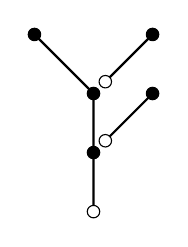
\begin{tikzpicture}[baseline=4ex, scale=.75]
		%% edges
		\draw[thick] (0,0) -- (0,1) -- (0,2) -- (-1,3);
		\draw[thick] (0.2,2.2) -- (1,3);
		\draw[thick] (0.2,1.2) -- (1,2);		
		%% vertices
		\draw[fill=white] (0,0) circle (3pt);
		\draw[fill=black] (0,1) circle (3pt);
		\draw[fill=white] (0.2,1.2) circle (3pt);
		\draw[fill=black] (0,2) circle (3pt);
		\draw[fill=white] (0.2,2.2) circle (3pt);
		\draw[fill=black] (-1,3) circle (3pt);
		\draw[fill=black] (1,3) circle (3pt);
		\draw[fill=black] (1,2) circle (3pt);
	 \end{tikzpicture} & 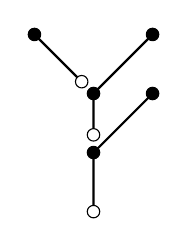
\begin{tikzpicture}[baseline=4ex, scale=.75]
		%% edges
		\draw[thick] (0,0) -- (0,1) -- (1,2);
		\draw[thick] (0,1.2) -- (0,2) -- (1,3);
		\draw[thick] (-0.2,2.2) -- (-1,3);
		%% vertices
		\draw[fill=white] (0,0) circle (3pt);
		\draw[fill=black] (0,1) circle (3pt);		
		\draw[fill=white] (0,1.3) circle (3pt);
		\draw[fill=black] (0,2) circle (3pt);
		\draw[fill=white] (-0.2,2.2) circle (3pt);
		\draw[fill=black] (-1,3) circle (3pt);
		\draw[fill=black] (1,3) circle (3pt);
		\draw[fill=black] (1,2) circle (3pt);
	\end{tikzpicture}\\
   ~& $\Updownarrow$ & $\Updownarrow$ \\
   $\displaystyle{val(\Gamma)}$ & $\displaystyle{
   		\leq \|S^3\| \|S\|^2
   	}$ & $\displaystyle{
   		\leq \|S^2\|^2 \|S\| {\color{gray} = \|S\|^5\left(\frac{\|S^2\|}{\|S\|^2}\right)^2}\!\!\!\!\!\!\!\!\!\!\!\!\!\!\!\!\!\!\!\!\!\!\!\!\!\!\!\!\!\!
   	}$
  \end{tabular}
\end{figure}
\end{adjustwidth}
\begin{wrapfigure}{l}{0pt}
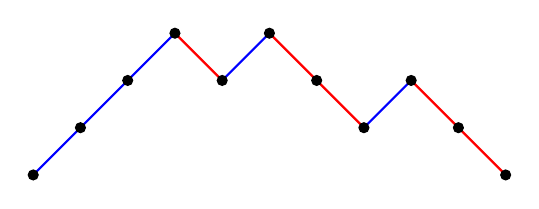
\begin{tikzpicture}[scale=.6]
	{\color{blue}\draw[thick] (0,0) -- (1,1) -- (2,2) -- (3,3);}
	{\color{red}\draw[thick] (3,3) -- (4,2);}
	{\color{blue}\draw[thick] (4,2) -- (5,3);}
	{\color{red}\draw[thick] (5,3) -- (6,2) -- (7,1);}
	{\color{blue}\draw[thick] (7,1) -- (8,2);}
	{\color{red}\draw[thick] (8,2) -- (9,1) -- (10,0);}
	%% vertices
	\draw[fill=black] (0,0) circle (3pt);
	\draw[fill=black] (1,1) circle (3pt);
	\draw[fill=black] (2,2) circle (3pt);
	\draw[fill=black] (3,3) circle (3pt);
	\draw[fill=black] (4,2) circle (3pt);
	\draw[fill=black] (5,3) circle (3pt);
	\draw[fill=black] (6,2) circle (3pt);
	\draw[fill=black] (7,1) circle (3pt);
	\draw[fill=black] (8,2) circle (3pt);
	\draw[fill=black] (9,1) circle (3pt);
	\draw[fill=black] (10,0) circle (3pt);	
\end{tikzpicture}\end{wrapfigure}
Count either {\color{blue}up-runs} or \emph{down-runs}. Every $j$-run improves the trivial bound $val(\Gamma)\leq \|S\|^n$ by a factor of $z_j\eqbydef \|S^j\|/\|S\|^j\leq 1$.

\bemph{Long runs improve our bound} since $\|S^j\|\leq \|S\|^j$ hardly ever saturates and gets better the bigger $j$ by submultiplicativity of $\|\cdot\|$.
\end{frame}

\begin{frame}
\frametitle{Bounds obtained by left- and rightmost splittings}
% in the paper we actually want to use the up-runs below some threshold \ell and the down-runs above this threshold - we have to be careful not to count both up- and down-runs at the same height, but this can be taken care of using the Pigeonhole principle
% note how the z_j encodes the factor of improvement over the trivial bound (corresponding to a complete splitting of the tree)
Under this identification of $\mathcal T_n\leftrightarrow D_{2n} : \Gamma\mapsto \pi(\Gamma)$, this yields the following bounds:
\begin{itemize}
	\item[\small leftmost:] $val(\pi(\Gamma)) \leq \|S\|^n \prod_i z_j^{\#j\text{-up-runs}(\pi(\Gamma))} =: \|S\|^n\; {\bf z}^{{\bf U}(\pi)}$
	\item[\small rightmost:] $val(\pi(\Gamma)) \leq \|S\|^n \prod_i z_j^{\#j\text{-down-runs}(\pi(\Gamma))} =: \|S\|^n\; {\bf z}^{{\bf D}(\pi)}$
	\item[\small mixture:] above height $\ell$ take rightmost splitting, below $\ell$ leftmost:
	\hspace*{-1cm}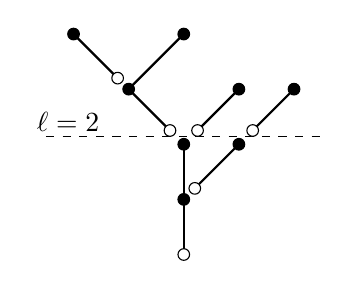
\begin{tikzpicture}[scale=.7, baseline=8ex]
		%% edges
		\draw[thick] (0,0) -- (0,1) -- (0,2);
		\draw[thick] (0.2,1.2) -- (1,2);
		\draw[thick] (1.25,2.25) -- (2,3);
		\draw[thick] (0.25,2.25) -- (1,3);
		\draw[thick] (-0.25,2.25) -- (-1,3) -- (0,4);
		\draw[thick] (-1.2,3.2) -- (-2,4);
		\draw[dashed] (-2.5,2.135) -- (2.5,2.135);
		%% vertices
		\draw[fill=white] (0,0) circle (3pt);
		\draw[fill=black] (0,1) circle (3pt);
		\draw[fill=white] (0.2,1.2) circle (3pt);
		\draw[fill=black] (0,2) circle (3pt);
		\draw[fill=white] (-0.25,2.25) circle (3pt);
		\draw[fill=white] (0.25, 2.25) circle (3pt);
		\draw[fill=black] (1,2) circle (3pt);
		\draw[fill=white] (1.25,2.25) circle (3pt);
		\draw[fill=black] (2,3) circle (3pt);
		\draw[fill=black] (1,3) circle (3pt);
		\draw[fill=black] (-1,3) circle (3pt);
		\draw[fill=white] (-1.2,3.2) circle (3pt);
		\draw[fill=black] (-2,4) circle (3pt);
		\draw[fill=black] (0,4) circle (3pt);
		% labels
		\node at (-2.1,2.4) {$\ell=2$};
	\end{tikzpicture} %$\Leftrightarrow$
	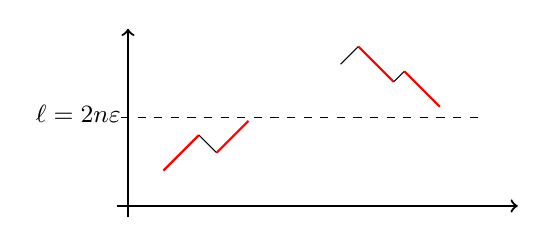
\begin{tikzpicture}[baseline=6ex,scale=.45]
		{\small \node at (-1.4,2.6) {$\ell=2n\e$};}

		\draw[->,thick] (-0.3,0)--(11,0);
		\draw[->,thick] (0,-0.3)--(0,5);
		\draw[dashed] (-0.2,2.5) -- (10,2.5);

		\draw[thin] (2,2) -- (2.5,1.5);
		\draw[thin] (6,4) -- (6.5,4.5);
		\draw[thin] (7.5,3.5) -- (7.8,3.8);
		{\color{red} 
			\draw[thick] (1,1) -- (2,2);
			\draw[thick] (2.5,1.5) -- (3.4,2.4);
			\draw[thick] (6.5,4.5) -- (7.5,3.5);
			\draw[thick] (7.8,3.8) -- (8.8,2.8);
		}
	\end{tikzpicture}
	
\end{itemize}\begin{itemize}
		\item Write $\|S\|^n\; {\bf z}^{{\bf T}_\ell(\pi)}$ for the bound obtained by this splitting.
		\item Have to be careful how to split around height $\ell$, but this can be controlled using the Pigeonhole principle.
	\end{itemize}
\end{frame}

\begin{frame}
\frametitle{Dyck paths as inhomogeneous Markov chains}
% analysing the distribution of the number of up-/down-runs of a given length under the uniform measure on the space of Dyck paths is made easier by the fact that we can generate a Dyck path by a Markov chain with explicit transition rates p_{t,h}
% we want to understand the energy landscape better
% note repulsive boundary conditions (repulsive at h=0, h=2k-t -> upper right triangle is particularly hard -> ignore it)
Fortunately, [Arnold 1980] showed that the uniform measure over $D_{2n}$ is induced by an \emph{inhomogeneous Markov chain} with $$p_{t,h}\deq\P\left(\pi(t+1)=h+1\, |\,\pi(t)=h\right)={\color<4-5>{red}\frac{1}{2}}{\color<4>{red}\frac{h+2}{h+1}}{\color<5>{red}\frac{2n-t-h}{2n-t}}.$$

	\begin{tikzpicture}[baseline=8ex, scale=.75]
		%% labels
		{\small
			\only<1>{\node at (5,2) {$p_{t,h}=??$};}
			\only<2>{\node at (10,2) {$2n-t, h$ small};}
			\only<3>{
				\node at (5,2) {$2n-t, h$ large};
				\node at (5,.5) {$2n-t$ large, $h$ small};				
			}
			\node at (11.3,0) {$t$};
			\node at (0,5.3) {$h$};
			\node at (10,-0.3) {$2n$};
			\only<2->{\node at (9.3,5.4) {$t=2n(1-\delta)$};}
			\only<3->{\node at (-1.2,1) {$2n\e=\ell$};}
			
			\only<4->{\node at (5,2.1) {$p_{t,h}\approx \frac{1}{2}\frac{2n-t-h}{2n-t}< \frac{1}{2}$};}
			\only<4->{\node at (5,0.5) {$p_{t,h}\approx \frac{1}{2}\frac{h+2}{h+1}>\frac{1}{2}$};}
		}
		
		%%% edges
		% coordinate axes
		\draw[->,thick] (-0.3,0)--(11,0);
		\draw[->,thick] (0,-0.3)--(0,5);
		
		% draw boundary of domain of p_{t,h}
		\draw[thin] (0,0) -- (5,5) -- (10,0);
		
		% draw boundaries between different cases
		\only<2->{\draw[dashed] (7.8,-0.25) -- (7.8,5.5);}
		\only<3->{\draw[dashed] (-0.25,1) -- (10.5,1);}
		
		% draw annotations
		\only<2>{\draw[->,thin] (9.8,1.8)--(8.65,.65);}
	\end{tikzpicture}

\end{frame}

\begin{frame}
\frametitle{How to bound $\E val(\pi(\Gamma))$}
% this is where the weird \phi_J from before comes from!
% considering only "tiny" segments of the path, we can approximate by transition probabilities that are more tractable
\emph{Under the simple random walk} ($\E_\frac{1}{2}$) of length $2n\to\infty$ we have the explicit formula (by [Holst 2014] and Cauchy Hadamard):
$$\limsup_{n\to\infty}\E_\frac{1}{2}\prod_{i\leq J} z_j^{\#j\text{-up-runs}(\pi)} \eqby{!} w_c(J)\quad \forall J\in\N$$
\emph{Markov property} allows us to chop up path (in time) in $1/\e$ ``small" segments $[t_j,t_{j+1}]\cap\N$.

	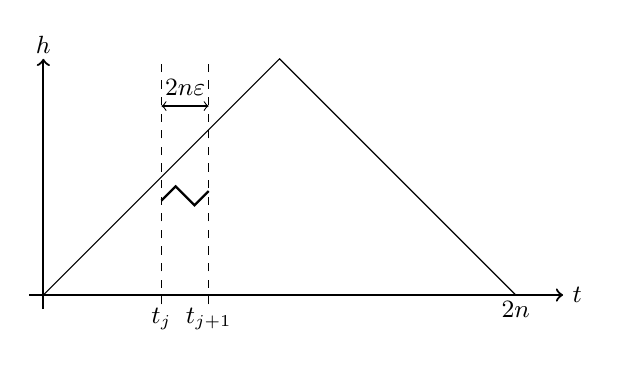
\begin{tikzpicture}[baseline=8ex, scale=.6]
		%% labels
		{\small
			\node at (11.3,0) {$t$};
			\node at (0,5.3) {$h$};
			\node at (10,-0.3) {$2n$};
			\node at (2.5,-0.5) {$t_j$};
			\node at (3.5,-0.5) {$t_{j+1}$};
			\node at (3,4.4) {$2n\e$};
		}
		%%% edges
		% coordinate axes
		\draw[->,thick] (-0.3,0)--(11,0);
		\draw[->,thick] (0,-0.3)--(0,5);
		
		% draw boundary of domain of p_{t,h}
		\draw[thin] (0,0) -- (5,5) -- (10,0);
		
		\draw[thick] (2.5,2)--(2.8,2.3)--(3.2,1.9)--(3.5,2.2);

		\draw[<->,thin] (2.5,4)--(3.5,4);
		\draw[dashed] (2.5,-.2) -- (2.5,5);
		\draw[dashed] (3.5,-.2) -- (3.5,5);
	\end{tikzpicture}

\end{frame}

\begin{frame}
\frametitle{Approximation by (time-)homogeneous Markov chain}
\begin{itemize}
	\item This allows us to \emph{approximate $p_{t,h}$} by ``nicer" rates $\tilde p_{t,h}$ such that
		$$\tilde p_{t,h}>\frac{1}{2}\text{ if }h\leq\ell\quad\text{and}\quad\tilde p_{t,h}<\frac{1}{2}\text{ if }h>\ell.$$
	\item \!\!\!Recall that ${\bf T}_\ell$ counted {\color{blue}up-runs if $h\leq \ell$} and \emph{down-runs if $h>\ell$}.\!\!\!\!\!\!
	\item \emph{Holley's inequality} and \emph{submultiplicativity of the norm} go in the right direction, i.e.
		$${\color{blue}\E_p {\bf z}^{\bf U} \le \E_\frac{1}{2} {\bf z}^{\bf U}}\quad\text{if }p>\frac{1}{2}\quad\text{and}\quad {\color{red}\E_p {\bf z}^{\bf D} \le \E_\frac{1}{2} {\bf z}^{\bf D}}\quad\text{if }p<\frac{1}{2},$$
		yielding (after taking $\lim_{\e,\delta\to 0}\limsup_{n\to\infty}$): $${\tiny\text{inverse factor of improvement = }}\E {\bf z}^{{\bf T}_\ell}\leq \E_\frac{1}{2}{\bf z}^{{\bf T}_\ell} = \E_\frac{1}{2}{\bf z}^{\bf U} {\tiny\text{ = known!}},$$ where $\E$ is expectation under uniform distribution of Dyck paths and $\E_\frac{1}{2}$ is expectation under the simple random walk.
\end{itemize}
\end{frame}

\section{Summary}

\begin{frame}
\frametitle{Summary}
\begin{itemize}
	\item We gave an explicit bound on the largest eigenvalue of a general Wigner type matrix in terms of the norm of the  matrix of variances $S$ and its powers.
	\item The solution of the corresponding deteministic equation (QVE) is expressed in terms of the statistics of up-runs and down-runs in the canonical Dyck-path ensemble.
	\item The inhomogeneous Markov chain behind the Dyck path ensemble can be approximated by a more tractable Markov chain, which, in turn, can be stochastically compared with the simple random walk (Holley inequality).
\end{itemize}


Thank you for your attention!
\end{frame}

%\begin{frame}
%\frametitle{Outlook: Where do we lose?}
%Actually the transition rates $\tilde p_{t,h}\deq\frac{1}{2}\frac{2n-t-h}{2n-t}<\frac{1}{2}$ are almost \emph{locally constant} (on a scale of $2n\e$), so that they would admit a (better) bound like $${\color{red}\E_{(t,h)}{\bf z}^{\bf D}\leq \E_{\tilde p_{t,h}}{\bf z}^{\bf D}} \,(<\E_\frac{1}{2}{\bf z}^{\bf D}).$$
%		
%Similarly for $\tilde p_{t,h}\deq\frac{1}{2}\frac{h+2}{h+1}>\frac{1}{2}$ for $h\approx 0$ (harder here).
%\\~\\		
%However, to make use of that gain we would \emph{need a better understanding of the paths}, in particular of how many paths cross any given point $(t,h)$ for large $n\gg 1$.
%\end{frame}

\begin{frame}
%\frametitle{Additional material}
\topskip0pt
\vspace*{\fill}
\hspace*{\fill}
{\huge\bemph{Additional material}}
\hspace*{\fill}
\vspace*{\fill}
\end{frame}

\begin{frame}
\frametitle{Holley's inequality (generalisation of FKG)}
\bemph{Setting} 
\begin{itemize}
	\item $\Omega\deq \{+1,-1\}^E$, with $E$ finite and $\omega\leq\omega'$ if $\omega(i)\leq\omega'(i)\;\forall i$
	\item $\P_1,\P_2$ probability measures on $\Omega$
	\item $X$ increasing, i.e. $\omega\leq \omega'\Rightarrow X(\omega)\leq X(\omega')$
\end{itemize}
\bemph{If}
\begin{enumerate}
	\item $\P_1(\omega^e)\P_2(\omega_e)\leq \P_1(\omega_e)\P_2(\omega^e)$, and
	\item for $\P$ being $\P_1$ or $\P_2$ one has $\P(\omega_{ef})\P(\omega^{ef})\geq \P(\omega^e_f)\P(\omega_e^f)$,
\end{enumerate}
where $\omega^e(t)\deq 1$, $\omega_e(t)\deq -1$ if $t=e$ and equal to $\omega$ else.

\bemph{Then}
$$\E_1 X\leq \E_2 X$$

\bemph{What we have to prove}
\begin{itemize}
	\item ${\bf z}^{{\bf D}(\omega_e)}\leq {\bf z}^{{\bf D}(\omega^e)}$
	\item $\P_{c<1/2}(\omega^e)\only<1>{\P_{\frac{1}{2}}(\omega_e)}\leq \P_{c<1/2}(\omega_e)\only<1>{\P_{\frac{1}{2}}(\omega^e)}$\only<2>{~}
\end{itemize}
\end{frame}

\end{document}
